\chapter{Results}
\label{chapter:results}

\section{Basic setup}
In the section we trained the model with the parameters described in the chapter \ref{chapter:methods}.
\subsection{YOLOv5}
The results of the YOLOv5 model for training and test dataset are available in the table \ref{tab:yolov5_basic}. To get further inside into the model, precision-recall curves for different intersection over union thresholds are ploted in the figure \ref{fig:yolov5_pr_curves}.
\begin{table}
    \begin{tabular}{c|c|c|c|c|c|c|c}
        stage & $AP$  & $AP@.3$ & $AP@.5$ & $AP@.75$ & $AP@.5_S$ & $AP@.5_M$ & $AP@.5_L$ \\ \hline
        train & 0.463 & 0.869   & 0.841   & 0.442    & 0.697     & 0.887     & 0.974     \\ \hline
        test  & 0.249 & 0.734   & 0.631   & 0.132    & 0.598     & 0.671     & 0.607     \\
    \end{tabular}
    \caption{Mean average precision of the YOLOv5 model}
    \label{tab:yolov5_basic}
\end{table}

\begin{paracol}{2}
    \begin{figure}
        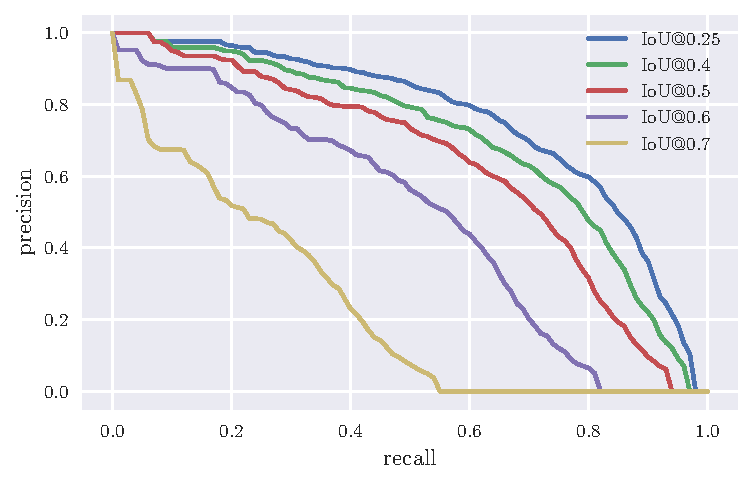
\includegraphics[width=\linewidth]{images/iou_val_multiple.pdf}
        \caption{Precision-recall curve of the YOLOv5 model}
        \label{fig:yolov5_pr_curves}
    \end{figure}
    \switchcolumn
    \begin{figure}
        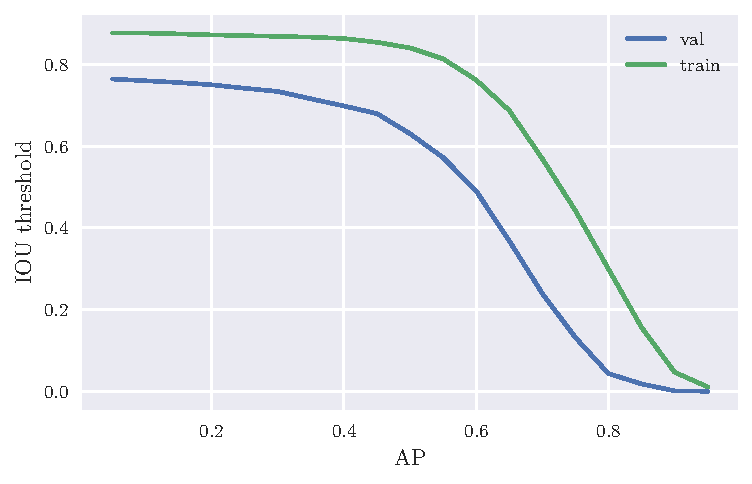
\includegraphics[width=\linewidth]{images/iou_threshold.pdf}
        \caption{The value of MAP based on the IOU threshold $\gamma$}
        \label{fig:yolov5_map_iou_thresholds}
    \end{figure}
\end{paracol}

\subsection{EfficientDet}


\section{Experiments}
The YOLOv5 model was selected, since it was the better perfoming one. Unless state otherwise, we kept the parameters as described in \ref{chapter:methods}. By a series of experiments, we tried to get insight into the importance of model parameters.
\subsection{Different backbones}
We changed the batch size to 2 (to be able to fit 5x6 backbone into the GPU memory) and trained the model with different backbones for 50 epochs each. Results for all runs are in the table \ref{tab:yolov5_backbones}.

\begin{table}
    \begin{tabular}{c|c|c|c|c|c}
        Backbone & $AP@.5$ & $AP$  & Parameters[M] & Flops[G] & Time[h] \\ \hline
        5s6      & 0.593   & 0.231 & 12            & 21       & 2.1     \\ \hline
        5m6      & 0.621   & 0.242 & 35            & 63       & 3.5     \\ \hline
        5l6      & 0.611   & 0.241 & 76            & 141      & 5.2     \\ \hline
        5x6      & 0.601   & 0.238 & 140           & 267      & 8.5     \\
    \end{tabular}
    \caption{Results of the YOLOv5 architecture with different backbones}
    \label{tab:yolov5_backbones}
\end{table}

\subsection{Different image size}
Once again, we kept the same setting and this time changed only the size to which images are resized. The relation between input image size and $AP@.5$ can be observed in the figure \ref{fig:img_sizes}.

\begin{paracol}{2}
    \begin{figure}
        \centering
        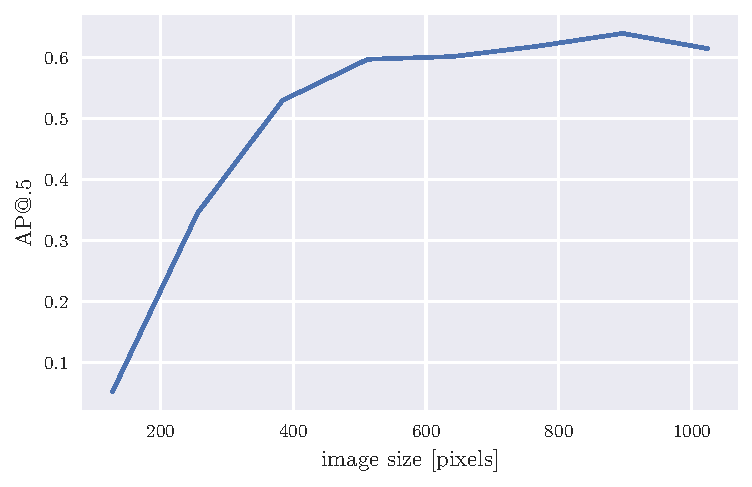
\includegraphics[width=0.99\linewidth]{images/img_size_dependency.pdf}
        \caption{The relation between image size and $AP@.5$}
        \label{fig:img_sizes}
    \end{figure}
    \switchcolumn
    \begin{figure}
        \centering
        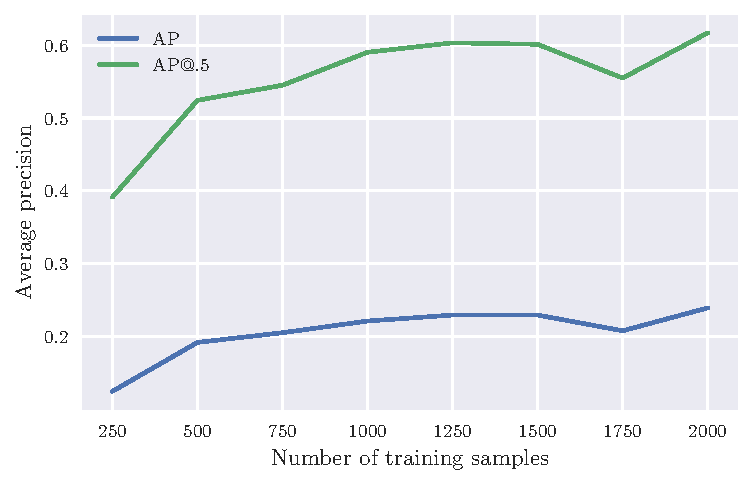
\includegraphics[width=0.99\linewidth]{images/training_set_dependency.pdf}
        \caption{Mean average precision based on the size of training set}
        \label{fig:training_set_sizes}
    \end{figure}
\end{paracol}


\subsection{Reduced training dataset}
We fixed the validation and test dataset and changed the amount of samples in the training dataset.

